\chapter{Evaluation}\label{cha:evaluation}

In this chapter, we will discuss our evaluation with the goal of answering the research questions in \Cref{cha:author-extraction}.

Three typical metrics for assessing the performance of a sequence tagging task are \gls{precision}, \gls{recall}, and the \gls{f1 score}~\citep{councill2008parscit}.
Given a sequence of words where each word is assigned a label out of a set of labels $L$, \gls{precision} and \gls{recall} are defined as~\citep{goutte2005probabilistic}:
\begin{equation*}
  \textit{precision}(L)=\frac{TP(L)}{TP(L)+FP(L)}\hspace{4em}\textit{recall}(L)=\frac{TP(L)}{TP(L)+FN(L)}
\end{equation*}
Here, $TP(L)$, $FP(L)$, and $FN(L)$ stand for the number of True Positive, False Positive, and False Negative assignments of labels in $L$, respectively.
Positive refers to the number words that are labeled with $L$ in the given tagged sequence and True refers to the number of words that are labeled with $L$ in a correctly tagged sequence.
Negative and False are defined accordingly.

To combine the two metrics into one, the \gls{f1 score} is defined as the harmonic mean of \gls{precision} and \gls{recall} \citep{bilenko2003adaptive}:
\begin{equation*}
  \textit{F1}(L)=\frac{2\cdot\textit{precision(L)}\cdot\textit{recall(L)}}{\textit{precision(L)}+\textit{recall(L)}}.
\end{equation*}

Further, we consider the metric of \gls{accuracy} which is defined as~\citep{powers2011evaluation}:
\begin{equation*}
  \textit{accuracy}(L)=\frac{TP(L)+TN(L)}{TP(L)+FP(L)+TN(L)+FN(L)}.
\end{equation*}
Yet, in \todo{ref} we show that the accuracy value of $L$ in our scenario always corresponds to the \gls{f1 score} calculated over all labels in $\textit{Val}$.
We will thereby not show the accuracy in our results.

\bigskip

To evaluate our models, a testing set of correctly tagged reference strings was manually created.
For this, we randomly selected $250$ \glspl{pdf} out of the \num{32470} research papers from \gls{ssoar}.
We were able to extract the text from $244$ \glspl{pdf}.
From this, we selected the $54$ research papers that satisfy the following requirements:
\begin{itemize}
  \item It is written in German.
  \item It contains a reference section.
  \item its text does not show signs of errors from the \gls{pdf} extraction step.
\end{itemize}

We then manually tagged all authors in the reference section, while also distinguishing between their first names and last names.
Statistics of the resulting labels for the \gls{bio} and \gls{bieo} formats are shown in \Cref{tab:statistics-manually-tagged}.
\begin{table}[t]
\centering
\begin{minipage}[t]{0.3\linewidth}
\centering
\gls{bio} Format\par
\smallskip
\begin{tabular}{l r}
  \toprule
  Label & Count\\
  \midrule
  \texttt{B-FN}    & \num{551}\\
  \texttt{B-LN}    & \num{2697}\\
                   & \\
                   & \\
  \texttt{I-FN}    & \num{3197}\\
  \texttt{I-LN}    & \num{609}\\
  \texttt{I-O}     & \num{1}\\
  \texttt{O}       & \num{33459}\\
  \midrule
  Author Labels    & \num{7055}\\
  All Labels       & \num{40514}\\
  \bottomrule
\end{tabular}
\end{minipage}
\quad
\begin{minipage}[t]{0.3\linewidth}
\centering
\gls{bieo} Format\par
\smallskip
\begin{tabular}{l r}
  \toprule
  Label & Count\\
  \midrule
  \texttt{B-FN}    & \num{551}\\
  \texttt{B-LN}    & \num{2697}\\
  \texttt{E-FN}    & \num{2655}\\
  \texttt{E-LN}    & \num{560}\\
  \texttt{I-FN}    & \num{542}\\
  \texttt{I-LN}    & \num{49}\\
  \texttt{I-O}     & \num{1}\\
  \texttt{O}       & \num{33459}\\
  \midrule
  Author Labels    & \num{7055}\\
  All Labels       & \num{40514}\\
  \bottomrule
\end{tabular}
\end{minipage}
\caption{Statistics on the manually tagged data set for labels following the \gls{bio} and \gls{bieo} format. ``Author Labels'' are ``All Labels'' minus the \texttt{O} labels.}
\label{tab:statistics-manually-tagged}
\end{table}
Note that our testing set contains exactly one word that has the label \texttt{I-O} for Intermediate Other.
This label is assigned to the misplaced comma in ``Wolff , S.'', which is part a reference string in \citet{morth1998spurensuche}.
Due to its relative insignificance, we do not consider this label in our learned model.

%\bigskip
%
Consequently, we exclude the manually tagged reference sections from the training set.
Due to the size of the training set, we only consider a randomly selected subset of reference sections for most of the evaluations.
When comparing training sets of different sizes, we do not ensure that the smaller training sets are a subset of the larger training sets.
Instead, every training subset is randomly extracted from the complete training set.

We now present our evaluations that address the individual research questions from \Cref{cha:author-extraction}.
Since we do not mention all parameters of our evaluation setup in the text, we refer to \todo{add} for more detailed information.

\bigskip

\RQ{1} considers the impact of using a related list of author names as the knowledge base in comparison to an unrelated list.
As discussed in \Cref{subsec:i-knowledge-base-creation}, we have two different sources of author names.
The \texttt{gnd} data set contains persons in the German speaking area but has no further restrictions on the research area.
The \texttt{swp} data set, on the other hand, contains author names that are related to the research area of our unlabeled set of reference sections.
To compare the two data sources, we additionally created the \texttt{swp-trim} data set.
It contains the same total number of authors as the \texttt{gnd} data set (see \Cref{tab:knowledge-base-statistics}).
\todo{consider gnd-diff vs gnd-full?}
In \todo{add}, we compare the precision and recall of the data sets for varying training set sizes.
The other parameters that were used in the experiments are summarized in \todo{add}.
\itodo{plots}

\bigskip

\RQ{2} aims at the performance differences between labelings in the \gls{bio} format and in the \gls{bieo} format.
In \Cref{sec:i-building-ge-constraints}, we showed that the \gls{bieo} format does not result in a more expressive author labeling than the \gls{bio} format.
Thereby, a direct comparison of the two formats is possible.

For our experiments, we use the \texttt{swp} data set and create labelings in the two different formats for both our training sets and manually labeled testing sets.
The results are shown in \todo{ref}.
\itodo{plots}

\bigskip

\RQ{3} addresses how the probability mass is assigned to a \gls{ge} constraint for words $w_n$ that are matched to no author name.
For this, we compare two approaches.
The first one is to assign the full probability mass of $1$ to the label \texttt{O}.
In the second approach, we only assign a specified part of the probability mass to label \texttt{O}.
The remaining probability mass is then distributed over all other labels.
Instead of specifying this distribution for all other labels, we derive it from our distantly supervised training set.
For example, we assume that the label \texttt{B-FN} was used in $25\%$ of all author labels in the distantly supervised training set.
Further, we specify that $80\%$ of our probability mass is assigned to the label \texttt{O}.
Therefore, we assign $25\%$ of the remaining $20\%$ of the probability mass to the label \texttt{B-FN}.

\itodo{plots}

\RQ{4} is focused on the ratio between matched and unmatched $w_n$ that are considered for building \gls{ge} constraints.
In \Cref{tab:ssoar-number-of-tags}, we summarize the number of tags that were assigned using our different knowledge bases.\todo{new table where we count matched and unmatched words}
As we can see, the percentage of\dots

\begin{table}[t]
  \centering
\begin{tabular}{c c c c c c}
 \toprule
 & \texttt{gnd-full} & \texttt{gnd-diff} &\texttt{swp-trim} &\texttt{swp-full} & \begin{tabular}[c]{@{}c@{}}\texttt{swp-full}\\+\texttt{gnd-full}\end{tabular} \\
 \midrule
 \texttt{AU} & \num{1161744} &  \num{958720} & \num{998163} &  \num{1203040} & \\
 \texttt{FN} & \num{1229106} & \num{1005942} & \num{1090405} & \num{1310711} & \\
 \texttt{LN} & \num{1167812} &  \num{961526} & \num{1003728} & \num{1210392} & \\
 \bottomrule
\end{tabular}
\caption{Number of \texttt{AU}, \texttt{FN}, and \texttt{LN} tags that were assigned to the \num{17294919} words in the \gls{ssoar} corpus using the different author name knowledge bases.}
\label{tab:ssoar-number-of-tags}
\end{table}

\Cref{fig:eval-other-ratios} shows the evaluation results for different ratios between unmatched words and matched words for the \gls{ge} constraints generation.
\begin{figure}[t]
\pgfplotsset{xlabel={\#Unmatched Words / \#Matched Words}}
\pgfplotsset{height=5.5cm,width=8cm}

\resizebox{\textwidth}{!}{%
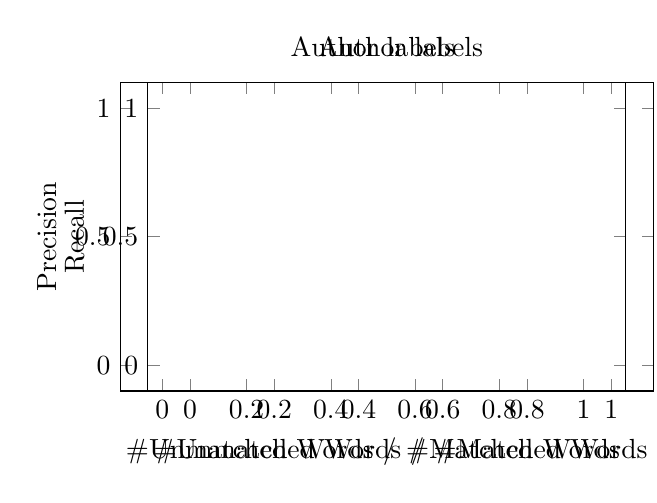
\begin{tikzpicture}
\begin{axis}[
    \firstchartconfig
    title={Author labels},
    ylabel={Precision},
    yticklabel style={/pgf/number format/precision=3},
    \colorlist
]
\plotfile{/home/martin/mt/plots/other-ratios-labels-precision.dat}
\legend{}; % empty the legend
\end{axis}

\hskip 10pt

\begin{axis}[
    \secondchartconfig
    \secondchartlegendconfig
    title={Author labels},
    ylabel={Recall},
    yticklabel style={/pgf/number format/precision=3},
    \colorlist
]
\plotfile{/home/martin/mt/plots/other-ratios-labels-recall.dat}
\end{axis}
\end{tikzpicture}
}

\vspace{10pt}

\resizebox{\textwidth}{!}{%
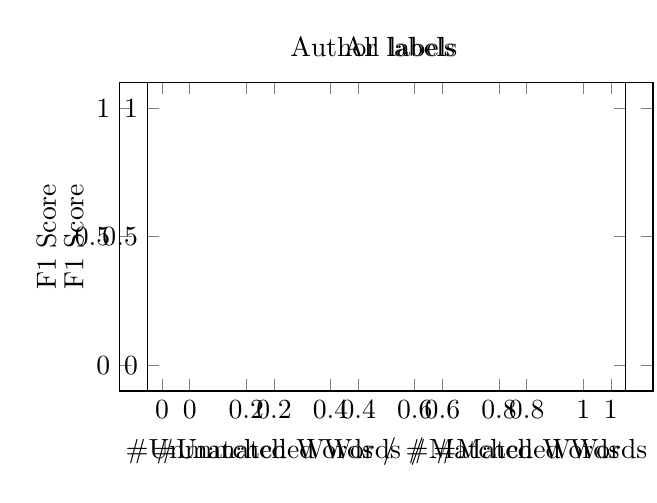
\begin{tikzpicture}
\begin{axis}[
    \firstchartconfig
    title={Author labels},
    ylabel={F1 Score},
    \colorlist
]
\plotfile{/home/martin/mt/plots/other-ratios-labels-f1.dat}
\legend{}; % empty the legend
\end{axis}

\hskip 10pt

\begin{axis}[
    \secondchartconfig
    title={All labels},
    ylabel={F1 Score},
    yticklabel style={/pgf/number format/precision=3},
    legend style={font=\ttfamily},
    \colorlist
]
\plotfile{/home/martin/mt/plots/other-ratios-total-f1.dat}
\legend{}; % empty the legend
\end{axis}
\end{tikzpicture}
}
\vspace*{-\baselineskip}

\caption{Evaluation results for different ratios between unmatched and matched words that are considered for building \gls{ge} constraints. 500, 1000, and 1500 correspond to the number of reference sections in the unlabeled data.}
\end{figure}
We can see that by increasing the relative amount of \texttt{O} from $0.5$ to $2.25$, the \gls{recall} for author labels decreases by almost $10\%$.
At the same time, the \gls{precision} of author labels does not linearly increase.
This is especially the case for the model that was learned of $1500$ reference sections.
When looking at the \gls{f1 score} of the author labels, we see for all three models that by increasing the ratio of \texttt{O} labels, the value first increases and then decreases.\todo{rewrite and remove \texttt{O} labels}
The more reference sections were used, the lower is the ratio of \texttt{O} labels that results in the best \gls{f1 score}.
The same is true when looking at the \gls{f1 score} of all labels.
When comparing the different models, we see that the bigger the model is, the smaller is the relative amount of \texttt{O} labels at the point with the highest \gls{f1 score}.

\bigskip

\RQ{5} considers a variation of the author extraction problem.
Instead of grouping words to individual author names and distinguishing between first and last names, a word $w_n$ is only labeled as part of an author name.
This results in a labeling which consists of two labels:
\texttt{A} for Author and \texttt{O} for Other.
We can directly derive this labeling from our more fine-grained approach.
For this, all labels that we use to denote a part of an author name, namely \texttt{B-FN}, \texttt{B-LN}, \texttt{I-FN}, and \texttt{I-LN}, are replaced with the label \texttt{A}.

In comparison to this, we also train separate models that only contain the two labels \texttt{A} and \texttt{O}.

\todo{add} compares the performance of these two approaches for the simplified author extraction problem.
\itodo{plots}

\bigskip

\RQ{6} focuses on the number of reference sections that are used in the unlabeled dataset $\mathcal{U}$ (see \Cref{subsec:generalized-expectation}).
Increasing the size of $\mathcal{U}$ also has an impact on the \gls{ge} constraints that are used in our model.
This is because \gls{ge} constraints are generated from matched author names in $\mathcal{U}$ against the external list of author names.

To address the research question, we generate several models with a varying number of reference sections in $\mathcal{U}$.
\itodo{plots}

\RQ{7} takes the Markov order of a \gls{linear-chain crf} into consideration.
\itodo{plots}

\bigskip


\RQ{8} aims to compare the impact of different regularization parameters of the Gaussian prior in a \gls{linear-chain crf} model.
%on gaussian prior: Additionally, \citet{sutton2010introduction} state that small changes to $\sigma^2$, for example up to a factor of 10, do not have a big impact on the accuracy of the final model.
%%sutton2010, page48: gauss=10 is typical for medium-sized training sets
\itodo{plots}

\bigskip

After addressing the research questions from \Cref{cha:author-extraction}, we now look into the hardware and time requirements of our approach.

First, we consider the main memory consumption of the learning process.
For this, we learn models with using a varying number of reference sections.
This changes both the size of the unlabeled data set as well as the number of \gls{ge} constraints.
In \todo{add} we show both the absolute increase in memory consumption as well as the increase per \todo{add}.



\itodo{plots}




